\subsection{Datasets}
The datasets for model evaluation includes 1500 images with more than 10000 different drugs. Each drug name is surrounded by a bounding box labeled with the correct drug name. Original images in our datasets have been downloaded from a Facebook group called "KHO DON THUOC"\footnote[1]{https://www.facebook.com/groups/392636900896314}, a small group created to gather prescriptions from all over the world and collected manually from large and small hospitals in the area. The manual check is conducted to ensure there is no duplication. 

Although the primary language of this datasets is Vietnamese, drug names are often scientific names, so they are less affected by Vietnamese punctuation or grammar. This datasets contains prescription images captured with the phone's camera, brightness or tilt angle subject to change. Although these conditions are similar to reality, they unintentionally create a big challenge for recognition models: how to accurately identify text under challenging conditions of brightness and tilt angle. Therefore, this datasets measure the accuracy and uptime of the prescription text recognition and detection system.

% The dataset for model evaluation includes 1500 images with more than 10000 different drugs. Each drug name is surrounded by a bounding box labeled with the correct drug name. This data set is collected from hospitals and websites that specialize in drugs.

% Although the primary language of this dataset is Vietnamese, drug names are often scientific names, so they are less affected by Vietnamese punctuation or grammar. This dataset contains prescription images captured with the phone's camera, brightness or tilt angle subject to change. Although these conditions are similar to reality, they unintentionally create a big challenge for recognition models: how to accurately identify text under challenging conditions of brightness and tilt angle. Therefore, this dataset measure the accuracy and uptime of the prescription text recognition and detection system. In the following sections, we describe collecting and labeling this dataset.

% Images in our dataset have been downloaded from a Facebook group called "KHO DON THUOC", a small group created to gather prescriptions from all over the world and collected manually from large and small hospitals in the area. We have done the checks to ensure there is no duplication.

% Most of the images in our dataset have been downloaded from a Facebook group called "KHO DON THUOC", which is a small group created to gather prescriptions from all over the world. In addition, many prescriptions were collected by us from large and small hospitals in the area. We have done the checks manually to ensure there is no duplication. The final dataset contains 1008 images from the Internet and 492 images collected and taken by team members from the hospital.

%A few images taken perform the sample labeling process to estimate a suitable process for the dataset. The bounding box is drawn around the text that is the drug name. The bounding box's coordinates and drug names were saved in a semi-structured text file (JSON). After completing the testing phase on the initial images, statistical techniques are applied to evaluate the labeling results then give out judgments about the labeling results to update the labeling process to improve the quality and consensus in the labeling results.

\subsection{Parameter settings}

This section features parameters and hardware for the proposed system in the experiment. For text detection, we modified CRAFT parameters: \(text\_threshold = 0.7\) and \(link\_threshold = 0.4\). We config sequence model VietOCR in recognition step to \(vgg\_seq2seq\). The threshold of MergeOCR is at 0.016, which determines the sensitivity of the clustering process. In medicine classifier, we set padding size to 300, filter size \(k = 2\), dilation factor \(d = [1, 2, 4]\). The medicine classifier threshold to confirm whether the text could be medicine is set to 0.6. Finally, the threshold to confirm and correct medicines is 0.85.
% We experiment with the whole proposed system in the same machine hardware, which has two core CPU Intel Xenon @2.20GHz, GPU Tesla K80 controlled by CUDA Version 11.2. 

\subsection{Evaluation Metrics}

Precision and recall are the major measurements we employ in the experiment. To assess the model's accuracy, an extra H-mean metric is also utilized. 
\begin{equation} \label{eq_precision}
   Precision = \frac{|\{accurate\;drugs\}\:\cap\:\{retrieved\;drugs\}|}{|\{retrieved\;drugs\}|}
\end{equation}
\begin{equation} \label{eq_recall}
   Recall = \frac{|\{accurate\;drugs\}\:\cap\:\{retrieved\;drugs\}|}{|\{accurate\;drugs\}|}
\end{equation}
\begin{equation} \label{eq_hmean}
   H{\text -}mean = 2\;\frac{Precision\:\cdot\:Recall}{Precision\:+\:Recall}
\end{equation}
Equation (\ref{eq_precision}), (\ref{eq_recall}), and (\ref{eq_hmean}) show the definition of Precision, Recall and H-mean. These metrics are used in the overall of the proposed prescription recognition system.
% Precision denotes the proportion of properly predicted drug names in the total
% output given by the system, whereas Recall shows the right prediction rate for
% all drug names in the data set. From the above two metrics, H-mean is also
% computed to evaluate the model’s quality in general.
\subsection{Result}
% Table 1 shows the experimental results after applying the introduced method. After the post-processing stage, the model achieves Precision and Recall of 0.94 and 0.73 respectively that increase by 0.4 and 0.56 points sequentially when compared to the model introduced by Nguyen et al. \cite{nguyen2021developing}.
Table ~\ref{tab1} shows the experimental results of new method and our old system \cite{nguyen2021developing}. The proposed model identifies effectively drug names in the data set, which outperforms the previous version with Precision and Recall up to 0.94 and 0.73, which increase by 0.4 and 0.56 respectively. However, the Recall score is just 0.73. In general, the cause is that the input data contains several errors. Simultaneously, the value of these metrics is heavily reliant on the medicines extraction step. This could be improved in the future if appropriate heuristic rules are implemented to make drug name extraction more efficient.
% \usepackage{siunitx}

\begin{table}
\centering
\caption{Evaluation on previous and upgraded system}\label{tab1}
% \begin{tabular}{|S[table-format=15.0]|S[table-format=10.2]|S[table-format=7.2]|S[table-format=7.2]|}
\begin{tabular}{|c|ccc|}
\hline
Model           & @Precision & @Recall & @H-mean  \\ 
\hline
Method in \cite{nguyen2021developing}      & 0.54       & 0.17    & 0.26     \\ 
\hline
\textbf{MEP} & \textbf{0.94}       & \textbf{0.73}    & \textbf{0.82}     \\
\hline
\end{tabular}
\end{table}

\begin{table}
\centering
\caption{The importance of medicine extractor in Prescription Recognition system}\label{tab2}
% \begin{tabular}{|S[table-format=15.0]|S[table-format=10.2]|S[table-format=7.2]|S[table-format=7.2]|}
\begin{tabular}{|c|c|c|c|c|}
\hline
Model           & OCRed text & MedicineExtractor & Spell correction & Output \\ 
\hline
Method in \cite{nguyen2021developing}      & Allpovic & - & [Alpovic]@0.9 & Alpovic     \\ 
\textbf{MEP} & Allpovic & \textbf{Allpovic} & [Alpovic]@0.9 & Alpovic     \\
\hline
Method in \cite{nguyen2021developing}      & Eperison 50mg (Macnir) & - & [Macnir]@0.6 & -      \\ 
\textbf{MEP} & Eperison 50mg (Macnir) & \textbf{Macnir} & [Macnir]@1.0 & Macnir     \\
\hline
\textbf{MEP} & Diovan 160mg (Valsartan) & \textbf{Diovan 160mg} & [Diovan 160]@0.94 & Diovan 160     \\
\hline
\end{tabular}
\end{table}
In addition, table~\ref{tab2} demonstrates how MEP achieves more stable results than the method in \cite{nguyen2021developing}. With the first medicine's name "Alpovic", both MEP and system in \cite{nguyen2021developing} work efficiently with high result confidence even though the inputs are misspelled. But when the output text of the OCR task is "Eperison 50mg (Macnir)", the old method can not separate drug and ingredient completely before applying it to the spell correction stage. As a result, the confidence metric is only 0.6, less than the configured threshold, so the model marks this text as non-drug. MEP overcome this restriction by adding a new layer to extract exactly drug names from the OCR stage, thanks to Medicine Classifier. No matter the complexity of OCRed text lines, the proposed method always knows which one is the drug name. In table~\ref{tab2}, MEP smoothly extracts "Macnir" and "Diovan 160mg" and throws them to the spell correction stage, finally achieving clear outcomes with excellent confidence. 

\begin{figure}
\centering
% 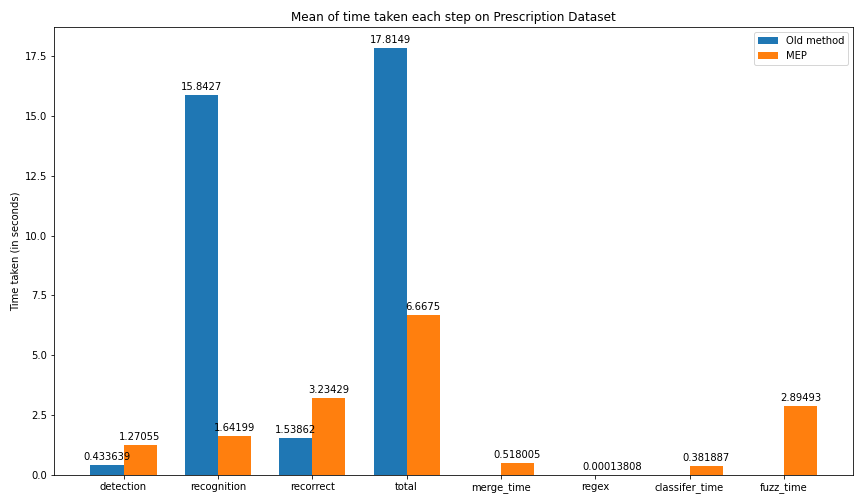
\includegraphics[width=0.7\textwidth]{experiment/barchart.png}
% 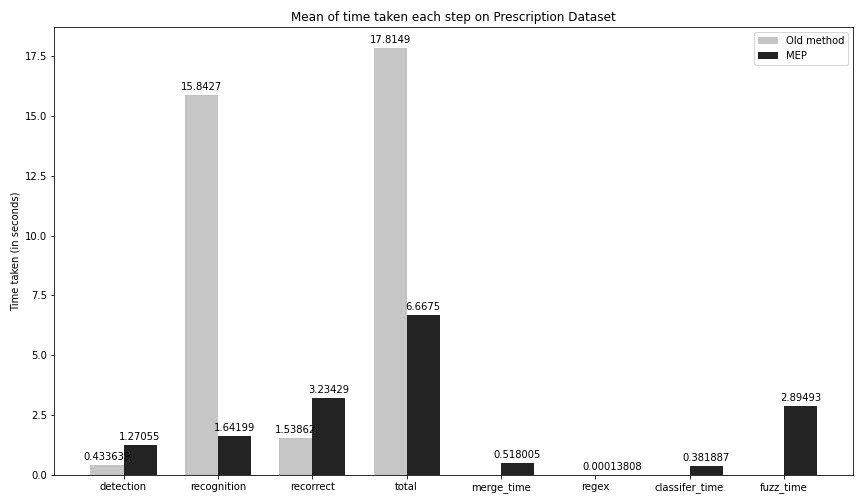
\includegraphics[width=0.7\textwidth]{experiment/charchart1.jpg}
\scalebox{0.55}{%% Creator: Matplotlib, PGF backend
%%
%% To include the figure in your LaTeX document, write
%%   \input{<filename>.pgf}
%%
%% Make sure the required packages are loaded in your preamble
%%   \usepackage{pgf}
%%
%% Also ensure that all the required font packages are loaded; for instance,
%% the lmodern package is sometimes necessary when using math font.
%%   \usepackage{lmodern}
%%
%% Figures using additional raster images can only be included by \input if
%% they are in the same directory as the main LaTeX file. For loading figures
%% from other directories you can use the `import` package
%%   \usepackage{import}
%%
%% and then include the figures with
%%   \import{<path to file>}{<filename>.pgf}
%%
%% Matplotlib used the following preamble
%%
\begingroup%
\makeatletter%
\begin{pgfpicture}%
\pgfpathrectangle{\pgfpointorigin}{\pgfqpoint{9.000000in}{5.000000in}}%
\pgfusepath{use as bounding box, clip}%
\begin{pgfscope}%
\pgfsetbuttcap%
\pgfsetmiterjoin%
\pgfsetlinewidth{0.000000pt}%
\definecolor{currentstroke}{rgb}{1.000000,1.000000,1.000000}%
\pgfsetstrokecolor{currentstroke}%
\pgfsetstrokeopacity{0.000000}%
\pgfsetdash{}{0pt}%
\pgfpathmoveto{\pgfqpoint{0.000000in}{0.000000in}}%
\pgfpathlineto{\pgfqpoint{9.000000in}{0.000000in}}%
\pgfpathlineto{\pgfqpoint{9.000000in}{5.000000in}}%
\pgfpathlineto{\pgfqpoint{0.000000in}{5.000000in}}%
\pgfpathlineto{\pgfqpoint{0.000000in}{0.000000in}}%
\pgfpathclose%
\pgfusepath{}%
\end{pgfscope}%
\begin{pgfscope}%
\pgfsetbuttcap%
\pgfsetmiterjoin%
\definecolor{currentfill}{rgb}{1.000000,1.000000,1.000000}%
\pgfsetfillcolor{currentfill}%
\pgfsetlinewidth{0.000000pt}%
\definecolor{currentstroke}{rgb}{0.000000,0.000000,0.000000}%
\pgfsetstrokecolor{currentstroke}%
\pgfsetstrokeopacity{0.000000}%
\pgfsetdash{}{0pt}%
\pgfpathmoveto{\pgfqpoint{0.516436in}{0.264771in}}%
\pgfpathlineto{\pgfqpoint{8.887500in}{0.264771in}}%
\pgfpathlineto{\pgfqpoint{8.887500in}{4.750662in}}%
\pgfpathlineto{\pgfqpoint{0.516436in}{4.750662in}}%
\pgfpathlineto{\pgfqpoint{0.516436in}{0.264771in}}%
\pgfpathclose%
\pgfusepath{fill}%
\end{pgfscope}%
\begin{pgfscope}%
\pgfpathrectangle{\pgfqpoint{0.516436in}{0.264771in}}{\pgfqpoint{8.371064in}{4.485891in}}%
\pgfusepath{clip}%
\pgfsetbuttcap%
\pgfsetmiterjoin%
\definecolor{currentfill}{rgb}{0.121569,0.466667,0.705882}%
\pgfsetfillcolor{currentfill}%
\pgfsetlinewidth{0.000000pt}%
\definecolor{currentstroke}{rgb}{0.000000,0.000000,0.000000}%
\pgfsetstrokecolor{currentstroke}%
\pgfsetstrokeopacity{0.000000}%
\pgfsetdash{}{0pt}%
\pgfpathmoveto{\pgfqpoint{0.896939in}{0.264771in}}%
\pgfpathlineto{\pgfqpoint{1.242850in}{0.264771in}}%
\pgfpathlineto{\pgfqpoint{1.242850in}{0.368763in}}%
\pgfpathlineto{\pgfqpoint{0.896939in}{0.368763in}}%
\pgfpathlineto{\pgfqpoint{0.896939in}{0.264771in}}%
\pgfpathclose%
\pgfusepath{fill}%
\end{pgfscope}%
\begin{pgfscope}%
\pgfpathrectangle{\pgfqpoint{0.516436in}{0.264771in}}{\pgfqpoint{8.371064in}{4.485891in}}%
\pgfusepath{clip}%
\pgfsetbuttcap%
\pgfsetmiterjoin%
\definecolor{currentfill}{rgb}{0.121569,0.466667,0.705882}%
\pgfsetfillcolor{currentfill}%
\pgfsetlinewidth{0.000000pt}%
\definecolor{currentstroke}{rgb}{0.000000,0.000000,0.000000}%
\pgfsetstrokecolor{currentstroke}%
\pgfsetstrokeopacity{0.000000}%
\pgfsetdash{}{0pt}%
\pgfpathmoveto{\pgfqpoint{1.885258in}{0.264771in}}%
\pgfpathlineto{\pgfqpoint{2.231170in}{0.264771in}}%
\pgfpathlineto{\pgfqpoint{2.231170in}{4.064071in}}%
\pgfpathlineto{\pgfqpoint{1.885258in}{4.064071in}}%
\pgfpathlineto{\pgfqpoint{1.885258in}{0.264771in}}%
\pgfpathclose%
\pgfusepath{fill}%
\end{pgfscope}%
\begin{pgfscope}%
\pgfpathrectangle{\pgfqpoint{0.516436in}{0.264771in}}{\pgfqpoint{8.371064in}{4.485891in}}%
\pgfusepath{clip}%
\pgfsetbuttcap%
\pgfsetmiterjoin%
\definecolor{currentfill}{rgb}{0.121569,0.466667,0.705882}%
\pgfsetfillcolor{currentfill}%
\pgfsetlinewidth{0.000000pt}%
\definecolor{currentstroke}{rgb}{0.000000,0.000000,0.000000}%
\pgfsetstrokecolor{currentstroke}%
\pgfsetstrokeopacity{0.000000}%
\pgfsetdash{}{0pt}%
\pgfpathmoveto{\pgfqpoint{2.873577in}{0.264771in}}%
\pgfpathlineto{\pgfqpoint{3.219489in}{0.264771in}}%
\pgfpathlineto{\pgfqpoint{3.219489in}{0.633754in}}%
\pgfpathlineto{\pgfqpoint{2.873577in}{0.633754in}}%
\pgfpathlineto{\pgfqpoint{2.873577in}{0.264771in}}%
\pgfpathclose%
\pgfusepath{fill}%
\end{pgfscope}%
\begin{pgfscope}%
\pgfpathrectangle{\pgfqpoint{0.516436in}{0.264771in}}{\pgfqpoint{8.371064in}{4.485891in}}%
\pgfusepath{clip}%
\pgfsetbuttcap%
\pgfsetmiterjoin%
\definecolor{currentfill}{rgb}{0.121569,0.466667,0.705882}%
\pgfsetfillcolor{currentfill}%
\pgfsetlinewidth{0.000000pt}%
\definecolor{currentstroke}{rgb}{0.000000,0.000000,0.000000}%
\pgfsetstrokecolor{currentstroke}%
\pgfsetstrokeopacity{0.000000}%
\pgfsetdash{}{0pt}%
\pgfpathmoveto{\pgfqpoint{3.861896in}{0.264771in}}%
\pgfpathlineto{\pgfqpoint{4.207808in}{0.264771in}}%
\pgfpathlineto{\pgfqpoint{4.207808in}{4.537048in}}%
\pgfpathlineto{\pgfqpoint{3.861896in}{4.537048in}}%
\pgfpathlineto{\pgfqpoint{3.861896in}{0.264771in}}%
\pgfpathclose%
\pgfusepath{fill}%
\end{pgfscope}%
\begin{pgfscope}%
\pgfpathrectangle{\pgfqpoint{0.516436in}{0.264771in}}{\pgfqpoint{8.371064in}{4.485891in}}%
\pgfusepath{clip}%
\pgfsetbuttcap%
\pgfsetmiterjoin%
\definecolor{currentfill}{rgb}{1.000000,0.498039,0.054902}%
\pgfsetfillcolor{currentfill}%
\pgfsetlinewidth{0.000000pt}%
\definecolor{currentstroke}{rgb}{0.000000,0.000000,0.000000}%
\pgfsetstrokecolor{currentstroke}%
\pgfsetstrokeopacity{0.000000}%
\pgfsetdash{}{0pt}%
\pgfpathmoveto{\pgfqpoint{1.242850in}{0.264771in}}%
\pgfpathlineto{\pgfqpoint{1.588762in}{0.264771in}}%
\pgfpathlineto{\pgfqpoint{1.588762in}{0.569467in}}%
\pgfpathlineto{\pgfqpoint{1.242850in}{0.569467in}}%
\pgfpathlineto{\pgfqpoint{1.242850in}{0.264771in}}%
\pgfpathclose%
\pgfusepath{fill}%
\end{pgfscope}%
\begin{pgfscope}%
\pgfpathrectangle{\pgfqpoint{0.516436in}{0.264771in}}{\pgfqpoint{8.371064in}{4.485891in}}%
\pgfusepath{clip}%
\pgfsetbuttcap%
\pgfsetmiterjoin%
\definecolor{currentfill}{rgb}{1.000000,0.498039,0.054902}%
\pgfsetfillcolor{currentfill}%
\pgfsetlinewidth{0.000000pt}%
\definecolor{currentstroke}{rgb}{0.000000,0.000000,0.000000}%
\pgfsetstrokecolor{currentstroke}%
\pgfsetstrokeopacity{0.000000}%
\pgfsetdash{}{0pt}%
\pgfpathmoveto{\pgfqpoint{2.231170in}{0.264771in}}%
\pgfpathlineto{\pgfqpoint{2.577081in}{0.264771in}}%
\pgfpathlineto{\pgfqpoint{2.577081in}{0.658542in}}%
\pgfpathlineto{\pgfqpoint{2.231170in}{0.658542in}}%
\pgfpathlineto{\pgfqpoint{2.231170in}{0.264771in}}%
\pgfpathclose%
\pgfusepath{fill}%
\end{pgfscope}%
\begin{pgfscope}%
\pgfpathrectangle{\pgfqpoint{0.516436in}{0.264771in}}{\pgfqpoint{8.371064in}{4.485891in}}%
\pgfusepath{clip}%
\pgfsetbuttcap%
\pgfsetmiterjoin%
\definecolor{currentfill}{rgb}{1.000000,0.498039,0.054902}%
\pgfsetfillcolor{currentfill}%
\pgfsetlinewidth{0.000000pt}%
\definecolor{currentstroke}{rgb}{0.000000,0.000000,0.000000}%
\pgfsetstrokecolor{currentstroke}%
\pgfsetstrokeopacity{0.000000}%
\pgfsetdash{}{0pt}%
\pgfpathmoveto{\pgfqpoint{3.219489in}{0.264771in}}%
\pgfpathlineto{\pgfqpoint{3.565401in}{0.264771in}}%
\pgfpathlineto{\pgfqpoint{3.565401in}{1.040398in}}%
\pgfpathlineto{\pgfqpoint{3.219489in}{1.040398in}}%
\pgfpathlineto{\pgfqpoint{3.219489in}{0.264771in}}%
\pgfpathclose%
\pgfusepath{fill}%
\end{pgfscope}%
\begin{pgfscope}%
\pgfpathrectangle{\pgfqpoint{0.516436in}{0.264771in}}{\pgfqpoint{8.371064in}{4.485891in}}%
\pgfusepath{clip}%
\pgfsetbuttcap%
\pgfsetmiterjoin%
\definecolor{currentfill}{rgb}{1.000000,0.498039,0.054902}%
\pgfsetfillcolor{currentfill}%
\pgfsetlinewidth{0.000000pt}%
\definecolor{currentstroke}{rgb}{0.000000,0.000000,0.000000}%
\pgfsetstrokecolor{currentstroke}%
\pgfsetstrokeopacity{0.000000}%
\pgfsetdash{}{0pt}%
\pgfpathmoveto{\pgfqpoint{4.207808in}{0.264771in}}%
\pgfpathlineto{\pgfqpoint{4.553720in}{0.264771in}}%
\pgfpathlineto{\pgfqpoint{4.553720in}{1.863732in}}%
\pgfpathlineto{\pgfqpoint{4.207808in}{1.863732in}}%
\pgfpathlineto{\pgfqpoint{4.207808in}{0.264771in}}%
\pgfpathclose%
\pgfusepath{fill}%
\end{pgfscope}%
\begin{pgfscope}%
\pgfpathrectangle{\pgfqpoint{0.516436in}{0.264771in}}{\pgfqpoint{8.371064in}{4.485891in}}%
\pgfusepath{clip}%
\pgfsetbuttcap%
\pgfsetmiterjoin%
\definecolor{currentfill}{rgb}{1.000000,0.498039,0.054902}%
\pgfsetfillcolor{currentfill}%
\pgfsetlinewidth{0.000000pt}%
\definecolor{currentstroke}{rgb}{0.000000,0.000000,0.000000}%
\pgfsetstrokecolor{currentstroke}%
\pgfsetstrokeopacity{0.000000}%
\pgfsetdash{}{0pt}%
\pgfpathmoveto{\pgfqpoint{5.196128in}{0.264771in}}%
\pgfpathlineto{\pgfqpoint{5.542039in}{0.264771in}}%
\pgfpathlineto{\pgfqpoint{5.542039in}{0.388995in}}%
\pgfpathlineto{\pgfqpoint{5.196128in}{0.388995in}}%
\pgfpathlineto{\pgfqpoint{5.196128in}{0.264771in}}%
\pgfpathclose%
\pgfusepath{fill}%
\end{pgfscope}%
\begin{pgfscope}%
\pgfpathrectangle{\pgfqpoint{0.516436in}{0.264771in}}{\pgfqpoint{8.371064in}{4.485891in}}%
\pgfusepath{clip}%
\pgfsetbuttcap%
\pgfsetmiterjoin%
\definecolor{currentfill}{rgb}{1.000000,0.498039,0.054902}%
\pgfsetfillcolor{currentfill}%
\pgfsetlinewidth{0.000000pt}%
\definecolor{currentstroke}{rgb}{0.000000,0.000000,0.000000}%
\pgfsetstrokecolor{currentstroke}%
\pgfsetstrokeopacity{0.000000}%
\pgfsetdash{}{0pt}%
\pgfpathmoveto{\pgfqpoint{6.184447in}{0.264771in}}%
\pgfpathlineto{\pgfqpoint{6.530359in}{0.264771in}}%
\pgfpathlineto{\pgfqpoint{6.530359in}{0.264804in}}%
\pgfpathlineto{\pgfqpoint{6.184447in}{0.264804in}}%
\pgfpathlineto{\pgfqpoint{6.184447in}{0.264771in}}%
\pgfpathclose%
\pgfusepath{fill}%
\end{pgfscope}%
\begin{pgfscope}%
\pgfpathrectangle{\pgfqpoint{0.516436in}{0.264771in}}{\pgfqpoint{8.371064in}{4.485891in}}%
\pgfusepath{clip}%
\pgfsetbuttcap%
\pgfsetmiterjoin%
\definecolor{currentfill}{rgb}{1.000000,0.498039,0.054902}%
\pgfsetfillcolor{currentfill}%
\pgfsetlinewidth{0.000000pt}%
\definecolor{currentstroke}{rgb}{0.000000,0.000000,0.000000}%
\pgfsetstrokecolor{currentstroke}%
\pgfsetstrokeopacity{0.000000}%
\pgfsetdash{}{0pt}%
\pgfpathmoveto{\pgfqpoint{7.172766in}{0.264771in}}%
\pgfpathlineto{\pgfqpoint{7.518678in}{0.264771in}}%
\pgfpathlineto{\pgfqpoint{7.518678in}{0.356353in}}%
\pgfpathlineto{\pgfqpoint{7.172766in}{0.356353in}}%
\pgfpathlineto{\pgfqpoint{7.172766in}{0.264771in}}%
\pgfpathclose%
\pgfusepath{fill}%
\end{pgfscope}%
\begin{pgfscope}%
\pgfpathrectangle{\pgfqpoint{0.516436in}{0.264771in}}{\pgfqpoint{8.371064in}{4.485891in}}%
\pgfusepath{clip}%
\pgfsetbuttcap%
\pgfsetmiterjoin%
\definecolor{currentfill}{rgb}{1.000000,0.498039,0.054902}%
\pgfsetfillcolor{currentfill}%
\pgfsetlinewidth{0.000000pt}%
\definecolor{currentstroke}{rgb}{0.000000,0.000000,0.000000}%
\pgfsetstrokecolor{currentstroke}%
\pgfsetstrokeopacity{0.000000}%
\pgfsetdash{}{0pt}%
\pgfpathmoveto{\pgfqpoint{8.161085in}{0.264771in}}%
\pgfpathlineto{\pgfqpoint{8.506997in}{0.264771in}}%
\pgfpathlineto{\pgfqpoint{8.506997in}{0.959016in}}%
\pgfpathlineto{\pgfqpoint{8.161085in}{0.959016in}}%
\pgfpathlineto{\pgfqpoint{8.161085in}{0.264771in}}%
\pgfpathclose%
\pgfusepath{fill}%
\end{pgfscope}%
\begin{pgfscope}%
\pgfsetbuttcap%
\pgfsetroundjoin%
\definecolor{currentfill}{rgb}{0.000000,0.000000,0.000000}%
\pgfsetfillcolor{currentfill}%
\pgfsetlinewidth{0.803000pt}%
\definecolor{currentstroke}{rgb}{0.000000,0.000000,0.000000}%
\pgfsetstrokecolor{currentstroke}%
\pgfsetdash{}{0pt}%
\pgfsys@defobject{currentmarker}{\pgfqpoint{0.000000in}{-0.048611in}}{\pgfqpoint{0.000000in}{0.000000in}}{%
\pgfpathmoveto{\pgfqpoint{0.000000in}{0.000000in}}%
\pgfpathlineto{\pgfqpoint{0.000000in}{-0.048611in}}%
\pgfusepath{stroke,fill}%
}%
\begin{pgfscope}%
\pgfsys@transformshift{1.242850in}{0.264771in}%
\pgfsys@useobject{currentmarker}{}%
\end{pgfscope}%
\end{pgfscope}%
\begin{pgfscope}%
\definecolor{textcolor}{rgb}{0.000000,0.000000,0.000000}%
\pgfsetstrokecolor{textcolor}%
\pgfsetfillcolor{textcolor}%
\pgftext[x=1.242850in,y=0.167548in,,top]{\color{textcolor}\rmfamily\fontsize{10.000000}{12.000000}\selectfont detection}%
\end{pgfscope}%
\begin{pgfscope}%
\pgfsetbuttcap%
\pgfsetroundjoin%
\definecolor{currentfill}{rgb}{0.000000,0.000000,0.000000}%
\pgfsetfillcolor{currentfill}%
\pgfsetlinewidth{0.803000pt}%
\definecolor{currentstroke}{rgb}{0.000000,0.000000,0.000000}%
\pgfsetstrokecolor{currentstroke}%
\pgfsetdash{}{0pt}%
\pgfsys@defobject{currentmarker}{\pgfqpoint{0.000000in}{-0.048611in}}{\pgfqpoint{0.000000in}{0.000000in}}{%
\pgfpathmoveto{\pgfqpoint{0.000000in}{0.000000in}}%
\pgfpathlineto{\pgfqpoint{0.000000in}{-0.048611in}}%
\pgfusepath{stroke,fill}%
}%
\begin{pgfscope}%
\pgfsys@transformshift{2.231170in}{0.264771in}%
\pgfsys@useobject{currentmarker}{}%
\end{pgfscope}%
\end{pgfscope}%
\begin{pgfscope}%
\definecolor{textcolor}{rgb}{0.000000,0.000000,0.000000}%
\pgfsetstrokecolor{textcolor}%
\pgfsetfillcolor{textcolor}%
\pgftext[x=2.231170in,y=0.167548in,,top]{\color{textcolor}\rmfamily\fontsize{10.000000}{12.000000}\selectfont recognition}%
\end{pgfscope}%
\begin{pgfscope}%
\pgfsetbuttcap%
\pgfsetroundjoin%
\definecolor{currentfill}{rgb}{0.000000,0.000000,0.000000}%
\pgfsetfillcolor{currentfill}%
\pgfsetlinewidth{0.803000pt}%
\definecolor{currentstroke}{rgb}{0.000000,0.000000,0.000000}%
\pgfsetstrokecolor{currentstroke}%
\pgfsetdash{}{0pt}%
\pgfsys@defobject{currentmarker}{\pgfqpoint{0.000000in}{-0.048611in}}{\pgfqpoint{0.000000in}{0.000000in}}{%
\pgfpathmoveto{\pgfqpoint{0.000000in}{0.000000in}}%
\pgfpathlineto{\pgfqpoint{0.000000in}{-0.048611in}}%
\pgfusepath{stroke,fill}%
}%
\begin{pgfscope}%
\pgfsys@transformshift{3.219489in}{0.264771in}%
\pgfsys@useobject{currentmarker}{}%
\end{pgfscope}%
\end{pgfscope}%
\begin{pgfscope}%
\definecolor{textcolor}{rgb}{0.000000,0.000000,0.000000}%
\pgfsetstrokecolor{textcolor}%
\pgfsetfillcolor{textcolor}%
\pgftext[x=3.219489in,y=0.167548in,,top]{\color{textcolor}\rmfamily\fontsize{10.000000}{12.000000}\selectfont recorrect}%
\end{pgfscope}%
\begin{pgfscope}%
\pgfsetbuttcap%
\pgfsetroundjoin%
\definecolor{currentfill}{rgb}{0.000000,0.000000,0.000000}%
\pgfsetfillcolor{currentfill}%
\pgfsetlinewidth{0.803000pt}%
\definecolor{currentstroke}{rgb}{0.000000,0.000000,0.000000}%
\pgfsetstrokecolor{currentstroke}%
\pgfsetdash{}{0pt}%
\pgfsys@defobject{currentmarker}{\pgfqpoint{0.000000in}{-0.048611in}}{\pgfqpoint{0.000000in}{0.000000in}}{%
\pgfpathmoveto{\pgfqpoint{0.000000in}{0.000000in}}%
\pgfpathlineto{\pgfqpoint{0.000000in}{-0.048611in}}%
\pgfusepath{stroke,fill}%
}%
\begin{pgfscope}%
\pgfsys@transformshift{4.207808in}{0.264771in}%
\pgfsys@useobject{currentmarker}{}%
\end{pgfscope}%
\end{pgfscope}%
\begin{pgfscope}%
\definecolor{textcolor}{rgb}{0.000000,0.000000,0.000000}%
\pgfsetstrokecolor{textcolor}%
\pgfsetfillcolor{textcolor}%
\pgftext[x=4.207808in,y=0.167548in,,top]{\color{textcolor}\rmfamily\fontsize{10.000000}{12.000000}\selectfont total}%
\end{pgfscope}%
\begin{pgfscope}%
\pgfsetbuttcap%
\pgfsetroundjoin%
\definecolor{currentfill}{rgb}{0.000000,0.000000,0.000000}%
\pgfsetfillcolor{currentfill}%
\pgfsetlinewidth{0.803000pt}%
\definecolor{currentstroke}{rgb}{0.000000,0.000000,0.000000}%
\pgfsetstrokecolor{currentstroke}%
\pgfsetdash{}{0pt}%
\pgfsys@defobject{currentmarker}{\pgfqpoint{0.000000in}{-0.048611in}}{\pgfqpoint{0.000000in}{0.000000in}}{%
\pgfpathmoveto{\pgfqpoint{0.000000in}{0.000000in}}%
\pgfpathlineto{\pgfqpoint{0.000000in}{-0.048611in}}%
\pgfusepath{stroke,fill}%
}%
\begin{pgfscope}%
\pgfsys@transformshift{5.196128in}{0.264771in}%
\pgfsys@useobject{currentmarker}{}%
\end{pgfscope}%
\end{pgfscope}%
\begin{pgfscope}%
\definecolor{textcolor}{rgb}{0.000000,0.000000,0.000000}%
\pgfsetstrokecolor{textcolor}%
\pgfsetfillcolor{textcolor}%
\pgftext[x=5.196128in,y=0.167548in,,top]{\color{textcolor}\rmfamily\fontsize{10.000000}{12.000000}\selectfont merge\_time}%
\end{pgfscope}%
\begin{pgfscope}%
\pgfsetbuttcap%
\pgfsetroundjoin%
\definecolor{currentfill}{rgb}{0.000000,0.000000,0.000000}%
\pgfsetfillcolor{currentfill}%
\pgfsetlinewidth{0.803000pt}%
\definecolor{currentstroke}{rgb}{0.000000,0.000000,0.000000}%
\pgfsetstrokecolor{currentstroke}%
\pgfsetdash{}{0pt}%
\pgfsys@defobject{currentmarker}{\pgfqpoint{0.000000in}{-0.048611in}}{\pgfqpoint{0.000000in}{0.000000in}}{%
\pgfpathmoveto{\pgfqpoint{0.000000in}{0.000000in}}%
\pgfpathlineto{\pgfqpoint{0.000000in}{-0.048611in}}%
\pgfusepath{stroke,fill}%
}%
\begin{pgfscope}%
\pgfsys@transformshift{6.184447in}{0.264771in}%
\pgfsys@useobject{currentmarker}{}%
\end{pgfscope}%
\end{pgfscope}%
\begin{pgfscope}%
\definecolor{textcolor}{rgb}{0.000000,0.000000,0.000000}%
\pgfsetstrokecolor{textcolor}%
\pgfsetfillcolor{textcolor}%
\pgftext[x=6.184447in,y=0.167548in,,top]{\color{textcolor}\rmfamily\fontsize{10.000000}{12.000000}\selectfont regex}%
\end{pgfscope}%
\begin{pgfscope}%
\pgfsetbuttcap%
\pgfsetroundjoin%
\definecolor{currentfill}{rgb}{0.000000,0.000000,0.000000}%
\pgfsetfillcolor{currentfill}%
\pgfsetlinewidth{0.803000pt}%
\definecolor{currentstroke}{rgb}{0.000000,0.000000,0.000000}%
\pgfsetstrokecolor{currentstroke}%
\pgfsetdash{}{0pt}%
\pgfsys@defobject{currentmarker}{\pgfqpoint{0.000000in}{-0.048611in}}{\pgfqpoint{0.000000in}{0.000000in}}{%
\pgfpathmoveto{\pgfqpoint{0.000000in}{0.000000in}}%
\pgfpathlineto{\pgfqpoint{0.000000in}{-0.048611in}}%
\pgfusepath{stroke,fill}%
}%
\begin{pgfscope}%
\pgfsys@transformshift{7.172766in}{0.264771in}%
\pgfsys@useobject{currentmarker}{}%
\end{pgfscope}%
\end{pgfscope}%
\begin{pgfscope}%
\definecolor{textcolor}{rgb}{0.000000,0.000000,0.000000}%
\pgfsetstrokecolor{textcolor}%
\pgfsetfillcolor{textcolor}%
\pgftext[x=7.172766in,y=0.167548in,,top]{\color{textcolor}\rmfamily\fontsize{10.000000}{12.000000}\selectfont classifer\_time}%
\end{pgfscope}%
\begin{pgfscope}%
\pgfsetbuttcap%
\pgfsetroundjoin%
\definecolor{currentfill}{rgb}{0.000000,0.000000,0.000000}%
\pgfsetfillcolor{currentfill}%
\pgfsetlinewidth{0.803000pt}%
\definecolor{currentstroke}{rgb}{0.000000,0.000000,0.000000}%
\pgfsetstrokecolor{currentstroke}%
\pgfsetdash{}{0pt}%
\pgfsys@defobject{currentmarker}{\pgfqpoint{0.000000in}{-0.048611in}}{\pgfqpoint{0.000000in}{0.000000in}}{%
\pgfpathmoveto{\pgfqpoint{0.000000in}{0.000000in}}%
\pgfpathlineto{\pgfqpoint{0.000000in}{-0.048611in}}%
\pgfusepath{stroke,fill}%
}%
\begin{pgfscope}%
\pgfsys@transformshift{8.161085in}{0.264771in}%
\pgfsys@useobject{currentmarker}{}%
\end{pgfscope}%
\end{pgfscope}%
\begin{pgfscope}%
\definecolor{textcolor}{rgb}{0.000000,0.000000,0.000000}%
\pgfsetstrokecolor{textcolor}%
\pgfsetfillcolor{textcolor}%
\pgftext[x=8.161085in,y=0.167548in,,top]{\color{textcolor}\rmfamily\fontsize{10.000000}{12.000000}\selectfont fuzz\_time}%
\end{pgfscope}%
\begin{pgfscope}%
\pgfsetbuttcap%
\pgfsetroundjoin%
\definecolor{currentfill}{rgb}{0.000000,0.000000,0.000000}%
\pgfsetfillcolor{currentfill}%
\pgfsetlinewidth{0.803000pt}%
\definecolor{currentstroke}{rgb}{0.000000,0.000000,0.000000}%
\pgfsetstrokecolor{currentstroke}%
\pgfsetdash{}{0pt}%
\pgfsys@defobject{currentmarker}{\pgfqpoint{-0.048611in}{0.000000in}}{\pgfqpoint{-0.000000in}{0.000000in}}{%
\pgfpathmoveto{\pgfqpoint{-0.000000in}{0.000000in}}%
\pgfpathlineto{\pgfqpoint{-0.048611in}{0.000000in}}%
\pgfusepath{stroke,fill}%
}%
\begin{pgfscope}%
\pgfsys@transformshift{0.516436in}{0.264771in}%
\pgfsys@useobject{currentmarker}{}%
\end{pgfscope}%
\end{pgfscope}%
\begin{pgfscope}%
\definecolor{textcolor}{rgb}{0.000000,0.000000,0.000000}%
\pgfsetstrokecolor{textcolor}%
\pgfsetfillcolor{textcolor}%
\pgftext[x=0.241744in, y=0.216545in, left, base]{\color{textcolor}\rmfamily\fontsize{10.000000}{12.000000}\selectfont \(\displaystyle {0.0}\)}%
\end{pgfscope}%
\begin{pgfscope}%
\pgfsetbuttcap%
\pgfsetroundjoin%
\definecolor{currentfill}{rgb}{0.000000,0.000000,0.000000}%
\pgfsetfillcolor{currentfill}%
\pgfsetlinewidth{0.803000pt}%
\definecolor{currentstroke}{rgb}{0.000000,0.000000,0.000000}%
\pgfsetstrokecolor{currentstroke}%
\pgfsetdash{}{0pt}%
\pgfsys@defobject{currentmarker}{\pgfqpoint{-0.048611in}{0.000000in}}{\pgfqpoint{-0.000000in}{0.000000in}}{%
\pgfpathmoveto{\pgfqpoint{-0.000000in}{0.000000in}}%
\pgfpathlineto{\pgfqpoint{-0.048611in}{0.000000in}}%
\pgfusepath{stroke,fill}%
}%
\begin{pgfscope}%
\pgfsys@transformshift{0.516436in}{0.864306in}%
\pgfsys@useobject{currentmarker}{}%
\end{pgfscope}%
\end{pgfscope}%
\begin{pgfscope}%
\definecolor{textcolor}{rgb}{0.000000,0.000000,0.000000}%
\pgfsetstrokecolor{textcolor}%
\pgfsetfillcolor{textcolor}%
\pgftext[x=0.241744in, y=0.816081in, left, base]{\color{textcolor}\rmfamily\fontsize{10.000000}{12.000000}\selectfont \(\displaystyle {2.5}\)}%
\end{pgfscope}%
\begin{pgfscope}%
\pgfsetbuttcap%
\pgfsetroundjoin%
\definecolor{currentfill}{rgb}{0.000000,0.000000,0.000000}%
\pgfsetfillcolor{currentfill}%
\pgfsetlinewidth{0.803000pt}%
\definecolor{currentstroke}{rgb}{0.000000,0.000000,0.000000}%
\pgfsetstrokecolor{currentstroke}%
\pgfsetdash{}{0pt}%
\pgfsys@defobject{currentmarker}{\pgfqpoint{-0.048611in}{0.000000in}}{\pgfqpoint{-0.000000in}{0.000000in}}{%
\pgfpathmoveto{\pgfqpoint{-0.000000in}{0.000000in}}%
\pgfpathlineto{\pgfqpoint{-0.048611in}{0.000000in}}%
\pgfusepath{stroke,fill}%
}%
\begin{pgfscope}%
\pgfsys@transformshift{0.516436in}{1.463842in}%
\pgfsys@useobject{currentmarker}{}%
\end{pgfscope}%
\end{pgfscope}%
\begin{pgfscope}%
\definecolor{textcolor}{rgb}{0.000000,0.000000,0.000000}%
\pgfsetstrokecolor{textcolor}%
\pgfsetfillcolor{textcolor}%
\pgftext[x=0.241744in, y=1.415616in, left, base]{\color{textcolor}\rmfamily\fontsize{10.000000}{12.000000}\selectfont \(\displaystyle {5.0}\)}%
\end{pgfscope}%
\begin{pgfscope}%
\pgfsetbuttcap%
\pgfsetroundjoin%
\definecolor{currentfill}{rgb}{0.000000,0.000000,0.000000}%
\pgfsetfillcolor{currentfill}%
\pgfsetlinewidth{0.803000pt}%
\definecolor{currentstroke}{rgb}{0.000000,0.000000,0.000000}%
\pgfsetstrokecolor{currentstroke}%
\pgfsetdash{}{0pt}%
\pgfsys@defobject{currentmarker}{\pgfqpoint{-0.048611in}{0.000000in}}{\pgfqpoint{-0.000000in}{0.000000in}}{%
\pgfpathmoveto{\pgfqpoint{-0.000000in}{0.000000in}}%
\pgfpathlineto{\pgfqpoint{-0.048611in}{0.000000in}}%
\pgfusepath{stroke,fill}%
}%
\begin{pgfscope}%
\pgfsys@transformshift{0.516436in}{2.063377in}%
\pgfsys@useobject{currentmarker}{}%
\end{pgfscope}%
\end{pgfscope}%
\begin{pgfscope}%
\definecolor{textcolor}{rgb}{0.000000,0.000000,0.000000}%
\pgfsetstrokecolor{textcolor}%
\pgfsetfillcolor{textcolor}%
\pgftext[x=0.241744in, y=2.015152in, left, base]{\color{textcolor}\rmfamily\fontsize{10.000000}{12.000000}\selectfont \(\displaystyle {7.5}\)}%
\end{pgfscope}%
\begin{pgfscope}%
\pgfsetbuttcap%
\pgfsetroundjoin%
\definecolor{currentfill}{rgb}{0.000000,0.000000,0.000000}%
\pgfsetfillcolor{currentfill}%
\pgfsetlinewidth{0.803000pt}%
\definecolor{currentstroke}{rgb}{0.000000,0.000000,0.000000}%
\pgfsetstrokecolor{currentstroke}%
\pgfsetdash{}{0pt}%
\pgfsys@defobject{currentmarker}{\pgfqpoint{-0.048611in}{0.000000in}}{\pgfqpoint{-0.000000in}{0.000000in}}{%
\pgfpathmoveto{\pgfqpoint{-0.000000in}{0.000000in}}%
\pgfpathlineto{\pgfqpoint{-0.048611in}{0.000000in}}%
\pgfusepath{stroke,fill}%
}%
\begin{pgfscope}%
\pgfsys@transformshift{0.516436in}{2.662913in}%
\pgfsys@useobject{currentmarker}{}%
\end{pgfscope}%
\end{pgfscope}%
\begin{pgfscope}%
\definecolor{textcolor}{rgb}{0.000000,0.000000,0.000000}%
\pgfsetstrokecolor{textcolor}%
\pgfsetfillcolor{textcolor}%
\pgftext[x=0.172299in, y=2.614688in, left, base]{\color{textcolor}\rmfamily\fontsize{10.000000}{12.000000}\selectfont \(\displaystyle {10.0}\)}%
\end{pgfscope}%
\begin{pgfscope}%
\pgfsetbuttcap%
\pgfsetroundjoin%
\definecolor{currentfill}{rgb}{0.000000,0.000000,0.000000}%
\pgfsetfillcolor{currentfill}%
\pgfsetlinewidth{0.803000pt}%
\definecolor{currentstroke}{rgb}{0.000000,0.000000,0.000000}%
\pgfsetstrokecolor{currentstroke}%
\pgfsetdash{}{0pt}%
\pgfsys@defobject{currentmarker}{\pgfqpoint{-0.048611in}{0.000000in}}{\pgfqpoint{-0.000000in}{0.000000in}}{%
\pgfpathmoveto{\pgfqpoint{-0.000000in}{0.000000in}}%
\pgfpathlineto{\pgfqpoint{-0.048611in}{0.000000in}}%
\pgfusepath{stroke,fill}%
}%
\begin{pgfscope}%
\pgfsys@transformshift{0.516436in}{3.262448in}%
\pgfsys@useobject{currentmarker}{}%
\end{pgfscope}%
\end{pgfscope}%
\begin{pgfscope}%
\definecolor{textcolor}{rgb}{0.000000,0.000000,0.000000}%
\pgfsetstrokecolor{textcolor}%
\pgfsetfillcolor{textcolor}%
\pgftext[x=0.172299in, y=3.214223in, left, base]{\color{textcolor}\rmfamily\fontsize{10.000000}{12.000000}\selectfont \(\displaystyle {12.5}\)}%
\end{pgfscope}%
\begin{pgfscope}%
\pgfsetbuttcap%
\pgfsetroundjoin%
\definecolor{currentfill}{rgb}{0.000000,0.000000,0.000000}%
\pgfsetfillcolor{currentfill}%
\pgfsetlinewidth{0.803000pt}%
\definecolor{currentstroke}{rgb}{0.000000,0.000000,0.000000}%
\pgfsetstrokecolor{currentstroke}%
\pgfsetdash{}{0pt}%
\pgfsys@defobject{currentmarker}{\pgfqpoint{-0.048611in}{0.000000in}}{\pgfqpoint{-0.000000in}{0.000000in}}{%
\pgfpathmoveto{\pgfqpoint{-0.000000in}{0.000000in}}%
\pgfpathlineto{\pgfqpoint{-0.048611in}{0.000000in}}%
\pgfusepath{stroke,fill}%
}%
\begin{pgfscope}%
\pgfsys@transformshift{0.516436in}{3.861984in}%
\pgfsys@useobject{currentmarker}{}%
\end{pgfscope}%
\end{pgfscope}%
\begin{pgfscope}%
\definecolor{textcolor}{rgb}{0.000000,0.000000,0.000000}%
\pgfsetstrokecolor{textcolor}%
\pgfsetfillcolor{textcolor}%
\pgftext[x=0.172299in, y=3.813759in, left, base]{\color{textcolor}\rmfamily\fontsize{10.000000}{12.000000}\selectfont \(\displaystyle {15.0}\)}%
\end{pgfscope}%
\begin{pgfscope}%
\pgfsetbuttcap%
\pgfsetroundjoin%
\definecolor{currentfill}{rgb}{0.000000,0.000000,0.000000}%
\pgfsetfillcolor{currentfill}%
\pgfsetlinewidth{0.803000pt}%
\definecolor{currentstroke}{rgb}{0.000000,0.000000,0.000000}%
\pgfsetstrokecolor{currentstroke}%
\pgfsetdash{}{0pt}%
\pgfsys@defobject{currentmarker}{\pgfqpoint{-0.048611in}{0.000000in}}{\pgfqpoint{-0.000000in}{0.000000in}}{%
\pgfpathmoveto{\pgfqpoint{-0.000000in}{0.000000in}}%
\pgfpathlineto{\pgfqpoint{-0.048611in}{0.000000in}}%
\pgfusepath{stroke,fill}%
}%
\begin{pgfscope}%
\pgfsys@transformshift{0.516436in}{4.461520in}%
\pgfsys@useobject{currentmarker}{}%
\end{pgfscope}%
\end{pgfscope}%
\begin{pgfscope}%
\definecolor{textcolor}{rgb}{0.000000,0.000000,0.000000}%
\pgfsetstrokecolor{textcolor}%
\pgfsetfillcolor{textcolor}%
\pgftext[x=0.172299in, y=4.413294in, left, base]{\color{textcolor}\rmfamily\fontsize{10.000000}{12.000000}\selectfont \(\displaystyle {17.5}\)}%
\end{pgfscope}%
\begin{pgfscope}%
\definecolor{textcolor}{rgb}{0.000000,0.000000,0.000000}%
\pgfsetstrokecolor{textcolor}%
\pgfsetfillcolor{textcolor}%
\pgftext[x=0.116744in,y=2.507716in,,bottom,rotate=90.000000]{\color{textcolor}\rmfamily\fontsize{10.000000}{12.000000}\selectfont Time taken (in seconds)}%
\end{pgfscope}%
\begin{pgfscope}%
\pgfsetrectcap%
\pgfsetmiterjoin%
\pgfsetlinewidth{0.803000pt}%
\definecolor{currentstroke}{rgb}{0.000000,0.000000,0.000000}%
\pgfsetstrokecolor{currentstroke}%
\pgfsetdash{}{0pt}%
\pgfpathmoveto{\pgfqpoint{0.516436in}{0.264771in}}%
\pgfpathlineto{\pgfqpoint{0.516436in}{4.750662in}}%
\pgfusepath{stroke}%
\end{pgfscope}%
\begin{pgfscope}%
\pgfsetrectcap%
\pgfsetmiterjoin%
\pgfsetlinewidth{0.803000pt}%
\definecolor{currentstroke}{rgb}{0.000000,0.000000,0.000000}%
\pgfsetstrokecolor{currentstroke}%
\pgfsetdash{}{0pt}%
\pgfpathmoveto{\pgfqpoint{8.887500in}{0.264771in}}%
\pgfpathlineto{\pgfqpoint{8.887500in}{4.750662in}}%
\pgfusepath{stroke}%
\end{pgfscope}%
\begin{pgfscope}%
\pgfsetrectcap%
\pgfsetmiterjoin%
\pgfsetlinewidth{0.803000pt}%
\definecolor{currentstroke}{rgb}{0.000000,0.000000,0.000000}%
\pgfsetstrokecolor{currentstroke}%
\pgfsetdash{}{0pt}%
\pgfpathmoveto{\pgfqpoint{0.516436in}{0.264771in}}%
\pgfpathlineto{\pgfqpoint{8.887500in}{0.264771in}}%
\pgfusepath{stroke}%
\end{pgfscope}%
\begin{pgfscope}%
\pgfsetrectcap%
\pgfsetmiterjoin%
\pgfsetlinewidth{0.803000pt}%
\definecolor{currentstroke}{rgb}{0.000000,0.000000,0.000000}%
\pgfsetstrokecolor{currentstroke}%
\pgfsetdash{}{0pt}%
\pgfpathmoveto{\pgfqpoint{0.516436in}{4.750662in}}%
\pgfpathlineto{\pgfqpoint{8.887500in}{4.750662in}}%
\pgfusepath{stroke}%
\end{pgfscope}%
\begin{pgfscope}%
\definecolor{textcolor}{rgb}{0.000000,0.000000,0.000000}%
\pgfsetstrokecolor{textcolor}%
\pgfsetfillcolor{textcolor}%
\pgftext[x=1.069895in,y=0.410430in,,bottom]{\color{textcolor}\rmfamily\fontsize{10.000000}{12.000000}\selectfont 0.433639}%
\end{pgfscope}%
\begin{pgfscope}%
\definecolor{textcolor}{rgb}{0.000000,0.000000,0.000000}%
\pgfsetstrokecolor{textcolor}%
\pgfsetfillcolor{textcolor}%
\pgftext[x=2.058214in,y=4.105738in,,bottom]{\color{textcolor}\rmfamily\fontsize{10.000000}{12.000000}\selectfont 15.8427}%
\end{pgfscope}%
\begin{pgfscope}%
\definecolor{textcolor}{rgb}{0.000000,0.000000,0.000000}%
\pgfsetstrokecolor{textcolor}%
\pgfsetfillcolor{textcolor}%
\pgftext[x=3.046533in,y=0.675421in,,bottom]{\color{textcolor}\rmfamily\fontsize{10.000000}{12.000000}\selectfont 1.53862}%
\end{pgfscope}%
\begin{pgfscope}%
\definecolor{textcolor}{rgb}{0.000000,0.000000,0.000000}%
\pgfsetstrokecolor{textcolor}%
\pgfsetfillcolor{textcolor}%
\pgftext[x=4.034852in,y=4.578714in,,bottom]{\color{textcolor}\rmfamily\fontsize{10.000000}{12.000000}\selectfont 17.8149}%
\end{pgfscope}%
\begin{pgfscope}%
\definecolor{textcolor}{rgb}{0.000000,0.000000,0.000000}%
\pgfsetstrokecolor{textcolor}%
\pgfsetfillcolor{textcolor}%
\pgftext[x=1.415806in,y=0.611134in,,bottom]{\color{textcolor}\rmfamily\fontsize{10.000000}{12.000000}\selectfont 1.27055}%
\end{pgfscope}%
\begin{pgfscope}%
\definecolor{textcolor}{rgb}{0.000000,0.000000,0.000000}%
\pgfsetstrokecolor{textcolor}%
\pgfsetfillcolor{textcolor}%
\pgftext[x=2.404126in,y=0.700209in,,bottom]{\color{textcolor}\rmfamily\fontsize{10.000000}{12.000000}\selectfont 1.64199}%
\end{pgfscope}%
\begin{pgfscope}%
\definecolor{textcolor}{rgb}{0.000000,0.000000,0.000000}%
\pgfsetstrokecolor{textcolor}%
\pgfsetfillcolor{textcolor}%
\pgftext[x=3.392445in,y=1.082065in,,bottom]{\color{textcolor}\rmfamily\fontsize{10.000000}{12.000000}\selectfont 3.23429}%
\end{pgfscope}%
\begin{pgfscope}%
\definecolor{textcolor}{rgb}{0.000000,0.000000,0.000000}%
\pgfsetstrokecolor{textcolor}%
\pgfsetfillcolor{textcolor}%
\pgftext[x=4.380764in,y=1.905398in,,bottom]{\color{textcolor}\rmfamily\fontsize{10.000000}{12.000000}\selectfont 6.6675}%
\end{pgfscope}%
\begin{pgfscope}%
\definecolor{textcolor}{rgb}{0.000000,0.000000,0.000000}%
\pgfsetstrokecolor{textcolor}%
\pgfsetfillcolor{textcolor}%
\pgftext[x=5.369083in,y=0.430662in,,bottom]{\color{textcolor}\rmfamily\fontsize{10.000000}{12.000000}\selectfont 0.518005}%
\end{pgfscope}%
\begin{pgfscope}%
\definecolor{textcolor}{rgb}{0.000000,0.000000,0.000000}%
\pgfsetstrokecolor{textcolor}%
\pgfsetfillcolor{textcolor}%
\pgftext[x=6.357403in,y=0.306470in,,bottom]{\color{textcolor}\rmfamily\fontsize{10.000000}{12.000000}\selectfont 0.00013808}%
\end{pgfscope}%
\begin{pgfscope}%
\definecolor{textcolor}{rgb}{0.000000,0.000000,0.000000}%
\pgfsetstrokecolor{textcolor}%
\pgfsetfillcolor{textcolor}%
\pgftext[x=7.345722in,y=0.398019in,,bottom]{\color{textcolor}\rmfamily\fontsize{10.000000}{12.000000}\selectfont 0.381887}%
\end{pgfscope}%
\begin{pgfscope}%
\definecolor{textcolor}{rgb}{0.000000,0.000000,0.000000}%
\pgfsetstrokecolor{textcolor}%
\pgfsetfillcolor{textcolor}%
\pgftext[x=8.334041in,y=1.000682in,,bottom]{\color{textcolor}\rmfamily\fontsize{10.000000}{12.000000}\selectfont 2.89493}%
\end{pgfscope}%
\begin{pgfscope}%
\definecolor{textcolor}{rgb}{0.000000,0.000000,0.000000}%
\pgfsetstrokecolor{textcolor}%
\pgfsetfillcolor{textcolor}%
\pgftext[x=4.701968in,y=4.833995in,,base]{\color{textcolor}\rmfamily\fontsize{12.000000}{14.400000}\selectfont Mean of time taken each step on Prescription Dataset}%
\end{pgfscope}%
\begin{pgfscope}%
\pgfsetbuttcap%
\pgfsetmiterjoin%
\definecolor{currentfill}{rgb}{1.000000,1.000000,1.000000}%
\pgfsetfillcolor{currentfill}%
\pgfsetfillopacity{0.800000}%
\pgfsetlinewidth{1.003750pt}%
\definecolor{currentstroke}{rgb}{0.800000,0.800000,0.800000}%
\pgfsetstrokecolor{currentstroke}%
\pgfsetstrokeopacity{0.800000}%
\pgfsetdash{}{0pt}%
\pgfpathmoveto{\pgfqpoint{7.450769in}{4.237544in}}%
\pgfpathlineto{\pgfqpoint{8.790278in}{4.237544in}}%
\pgfpathquadraticcurveto{\pgfqpoint{8.818056in}{4.237544in}}{\pgfqpoint{8.818056in}{4.265322in}}%
\pgfpathlineto{\pgfqpoint{8.818056in}{4.653439in}}%
\pgfpathquadraticcurveto{\pgfqpoint{8.818056in}{4.681217in}}{\pgfqpoint{8.790278in}{4.681217in}}%
\pgfpathlineto{\pgfqpoint{7.450769in}{4.681217in}}%
\pgfpathquadraticcurveto{\pgfqpoint{7.422992in}{4.681217in}}{\pgfqpoint{7.422992in}{4.653439in}}%
\pgfpathlineto{\pgfqpoint{7.422992in}{4.265322in}}%
\pgfpathquadraticcurveto{\pgfqpoint{7.422992in}{4.237544in}}{\pgfqpoint{7.450769in}{4.237544in}}%
\pgfpathlineto{\pgfqpoint{7.450769in}{4.237544in}}%
\pgfpathclose%
\pgfusepath{stroke,fill}%
\end{pgfscope}%
\begin{pgfscope}%
\pgfsetbuttcap%
\pgfsetmiterjoin%
\definecolor{currentfill}{rgb}{0.121569,0.466667,0.705882}%
\pgfsetfillcolor{currentfill}%
\pgfsetlinewidth{0.000000pt}%
\definecolor{currentstroke}{rgb}{0.000000,0.000000,0.000000}%
\pgfsetstrokecolor{currentstroke}%
\pgfsetstrokeopacity{0.000000}%
\pgfsetdash{}{0pt}%
\pgfpathmoveto{\pgfqpoint{7.478547in}{4.521495in}}%
\pgfpathlineto{\pgfqpoint{7.756325in}{4.521495in}}%
\pgfpathlineto{\pgfqpoint{7.756325in}{4.618717in}}%
\pgfpathlineto{\pgfqpoint{7.478547in}{4.618717in}}%
\pgfpathlineto{\pgfqpoint{7.478547in}{4.521495in}}%
\pgfpathclose%
\pgfusepath{fill}%
\end{pgfscope}%
\begin{pgfscope}%
\definecolor{textcolor}{rgb}{0.000000,0.000000,0.000000}%
\pgfsetstrokecolor{textcolor}%
\pgfsetfillcolor{textcolor}%
\pgftext[x=7.867436in,y=4.521495in,left,base]{\color{textcolor}\rmfamily\fontsize{10.000000}{12.000000}\selectfont Method in \cite{nguyen2021developing}}%
\end{pgfscope}%
\begin{pgfscope}%
\pgfsetbuttcap%
\pgfsetmiterjoin%
\definecolor{currentfill}{rgb}{1.000000,0.498039,0.054902}%
\pgfsetfillcolor{currentfill}%
\pgfsetlinewidth{0.000000pt}%
\definecolor{currentstroke}{rgb}{0.000000,0.000000,0.000000}%
\pgfsetstrokecolor{currentstroke}%
\pgfsetstrokeopacity{0.000000}%
\pgfsetdash{}{0pt}%
\pgfpathmoveto{\pgfqpoint{7.478547in}{4.320106in}}%
\pgfpathlineto{\pgfqpoint{7.756325in}{4.320106in}}%
\pgfpathlineto{\pgfqpoint{7.756325in}{4.417328in}}%
\pgfpathlineto{\pgfqpoint{7.478547in}{4.417328in}}%
\pgfpathlineto{\pgfqpoint{7.478547in}{4.320106in}}%
\pgfpathclose%
\pgfusepath{fill}%
\end{pgfscope}%
\begin{pgfscope}%
\definecolor{textcolor}{rgb}{0.000000,0.000000,0.000000}%
\pgfsetstrokecolor{textcolor}%
\pgfsetfillcolor{textcolor}%
\pgftext[x=7.867436in,y=4.320106in,left,base]{\color{textcolor}\rmfamily\fontsize{10.000000}{12.000000}\selectfont MEP}%
\end{pgfscope}%
\end{pgfpicture}%
\makeatother%
\endgroup%
}
\caption{Average processing time in stages}\label{fig_barchart}
\end{figure}

In terms of processing time, our model outperforms with the fastest and slowest processing times across the system at 1.38 seconds and 29.65 seconds, respectively, compared to 3.81 seconds and 51.24 seconds of the previous model. Fig.~\ref{fig_barchart} compares the average processing time of each step on the prescription datasets between the two versions. When Tesseract is replaced by VietOCR that speeds up time from 15.84 second to 1.64 seconds in average. This implies the application of the character recognition model depends on the characteristics of the problem being solved. MEP shortens the required time to match a string to a dictionary. Despite having a lexicon that is more than 100 times larger than the prior one, matching time rose by just 1.69 seconds on average when compared to the previous model.

Overall, the upgraded system has shown a significant improvement in all mentioned metrics. Despite some additional intermediate steps before dictionary matching, our total drug name recognition and the average extraction time is 6.67 seconds per prescription, compared to 17.81 seconds average processing times of the old model. That demonstrates the efficiency in terms of time and accuracy that our model achieves on the problem posed.
